\documentclass{article}
\usepackage{graphicx}
\usepackage{hyperref}
\usepackage[svgnames]{xcolor}
\usepackage{listings}

% some adjustments for the lstlisting environment used to typeset code
\lstset{backgroundcolor=\color{LightSteelBlue!60},
  frame=trbl,
  rulecolor=\color{black!30},
  xrightmargin=7pt}

\begin{document}
\title{Multicast Routing in Linux}
\author{Ang Way Chuang \\
\small{\href{mailto:wcang79@gmail.com}{wcang79@gmail.com}}}
\date{\today}
\maketitle
\section{Foreword}
This is part of an ongoing effort to understand how multicast forwarding works
and implementation of multicast routing within a routing daemon on Linux (UNIX)
system. Those who want to look for guide to write multicast application should
look elsewhere. As my understanding on multicast routing is quite limited,
errors are to be expected and the document will remain incomplete and
disorganized until I have a better understanding on the subject. I would like to
thank Afumado Basuki for his encouragement and his eargerness to share his
knowledge. You're my multicast routing god.

There are a lot of online references on PIM multicast routing, but there is
hardly any that discusses how it is implemented in Linux. This document tries to
address that gap. Each section will try to address the WHY first before diving
into the HOW. This document refers to the implementation of Linux kernel version
3, but the discussion should apply to older and newer kernels that implements
multicast routing. Due to time limit, this document shall limit itself to the
discussion of IPv6.

\section{Multicast Forwarding}
\begin{figure}[h]
  \begin{center}
    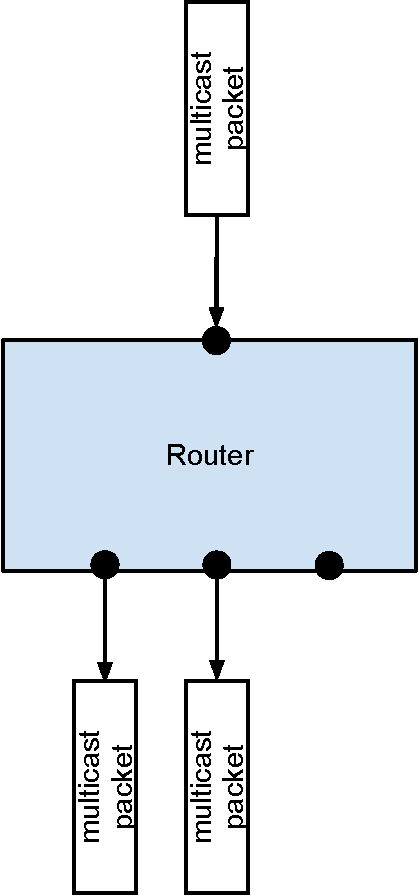
\includegraphics[width=0.3\textwidth]{mcast-forward}
    \caption{Router duplicates and send out multicast packet to the
    outgoing interfaces that have active listeners of multicast group}
    \label{fig:mcast-forward}
  \end{center}
\end{figure}

As shown in Figure \ref{fig:mcast-forward}, unlike unicast forwarding, when a
multicast packet is received by a router, the packet may be forwarded to
multiple outgoing interfaces. While, it is the job of the kernel to duplicate
the packet and forward the multicast packet to all the relevant outgoing
interfaces, the kernel doesn't know which interfaces to forward the multicast
packet. 

Routing daemon running PIM protocol will learn about the active listeners of the
multicast stream and therefore which outgoing interfaces where the multicast
packet should be forwarded. Therefore, it is the job of routing daemon to
instruct the kernel on this matter by adding multicast forwarding cache (MFC).

MFC basically consists of the following tuple:
\begin{itemize}
  \item source address - source (S) address of multicast packet
  \item group address - group (G) address of multicast packet
  \item incoming interface - the network interface where the multicast packet
  belonging to the (S,G) should be received. This information will be used for
  RPF checking within the kernel (\texttt{ip6\_mr\_forward}). RPF checking is
  done solely based on MFC entry. At first, it seems counter-intuitive to have
  this additional parameter as the kernel can perform RPF checking based on its
  routing table.  While the kernel has the required information to perform RPF
  checking based unicast Forwarding Information Base (FIB, or in other word,
  routing table), it doesn't know about the Multicast Forwarding Information
  Base (MFIB) because there is no corresponding FIB for multicast in the kernel.
  Only the multicast routing daemon has the information on MFIB. For typical
  deployment, most of the entries of MFIB corresponds to FIB as MFIB is mostly
  constructed from FIB. However, there are situation where it may differ. Apart
  from that, the incoming interface for a multicast stream may be different when
  the stream is delivered through Rendezvous Point Tree (RPT) and Shortest Path
  Tree (SPT). Therefore, the routing daemon may need to modify this parameter when
  it switches the multicast stream from RPT to SPT.
  \item list of outgoing interfaces - the list of network interfaces where the
  multicast packet belonging to (S,G) should be forwarded 
\end{itemize}

User space routing daemon can manipulate MFC using \texttt{mf6cctl\{\}}
(\texttt{<linux/mroute6.h>}). Within the kernel, MFC entry is represented by
\texttt{mfc6\_cache\{\}} (\texttt{include/linux/mroute6.h}).

The following subsections will highlight the multicast packet traversal process
for 2 MFC states:

\begin{itemize}
  \item unresolved (queued) state - Unresolved state only happens when there is
  no pre-installed (by routing daemon) MFC entry when a (S,G) multicast packet
  is received. In this case, the kernel will create an unresolved (or called
  queued) MFC entry for the multicast packet. In this state, multicast packet
  cannot be forwarded because it doesn't know the outgoing interfaces.
  \item resolved state - In this state, there is a matching MFC entry was to assist
  with the multicast forwarding. Most literature refers to this state when MFC
  is mentioned as unresolved MFC entry cannot be used to performed multicast
  forwarding.
\end{itemize}

 
\subsection{MFC States}

\begin{figure}[h]
  \begin{center}
    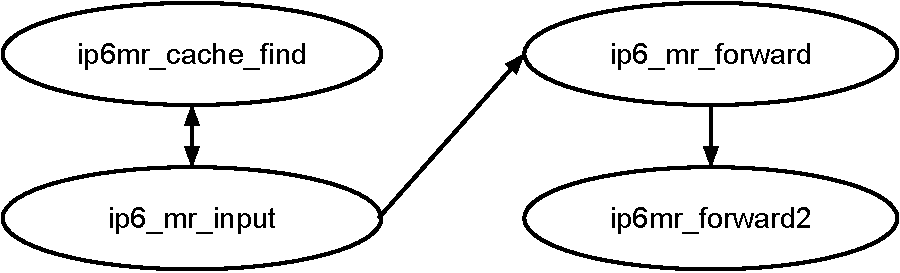
\includegraphics[width=\textwidth]{mcast-mfc}
    \caption{Interaction between kernel and user space routing daemon on the
    occassion of unresolved and resolved MFC states}
    \label{fig:mcast-unresolved}
  \end{center}
\end{figure}

Figure \ref{fig:mcast-unresolved} is the simplified interaction of kernel and
user space routing daemon in the process of forwarding multicast packet. Let's
begin with the resolved state as it is the simpler one. The processing of a
multicast packet begins with \texttt{ip6\_mr\_input}. \texttt{ip6\_mr\_input}
calls \texttt{ip6mr\_cache\_find} to lookup for a matching MFC entry based upon
the source and group addresses of the multicast packet. All resolved MFC entries
are stored in \texttt{mfc6\_cache\_array} list of \texttt{mr6\_table}.  Barring
the usage of namespace, typical deployment will only have single
\texttt{mr6\_table} to manage multicast forwarding. In the case of resolved
state, \texttt{mfc6\_cache\_find} will return a matching MFC entry. In which
case, \texttt{ip6\_mr\_input} will pass the packet directly to
\texttt{ip6\_mr\_forward}. For each outgoing interface that has active listener,
\texttt{ip6mr\_forward2} will be called to forward the packet to the interface.
\textit{Why IPv6 forwarding code uses hop limit to determine the forwarding?}

In the case of unresolved state, there will not be any matching MFC entry. The
packet will be passed to \texttt{ip6mr\_cache\_unresolved}.
\texttt{ip6mr\_cache\_unresolved} will create an unresolved MFC entry for the
packet if there is no prior unresolved MFC entry for this packet and enqueue the
packet into the MFC entry. All unresolved MFC entries are enqueued within the
\texttt{mfc6\_unres\_queue} list of \texttt{mr6\_table}.


\texttt{ip6mr\_cache\_unresolved} will call \texttt{ip6mr\_cache\_report}.
\texttt{ip6mr\_cache\_report} will create a packet to inform routing daemon of
the unresolved cache event using multicast socket. The packet is an IPv6 packet
with the following format in Figure \ref{fig:mcast-upcall}:

\begin{figure}[h]
  \begin{center}
    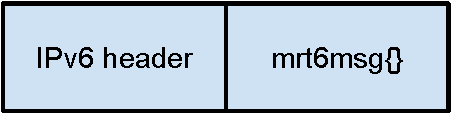
\includegraphics[width=0.4\textwidth]{mcast-upcall}
    \caption{Packet format of IPv6 multicast upcall}
    \label{fig:mcast-upcall}
  \end{center}
\end{figure}

\texttt{im6\_mif}, \texttt{im6\_src} and \texttt{im6\_dst} of
\texttt{mrt6msg\{\}} contains sufficient information for routing daemon to
determine the list of outgoing interfaces and install a corresponding MFC using
\texttt{setsockopt(fd, IPROTO\_IPV6, MRT6\_ADD\_MFC, \ldots)}. Corresponding to
that, kernel's \texttt{ip\_mroute\_setsockopt} will call
\texttt{ip6mr\_mfc\_add} to add a new MFC (resolved) entry and remove the
corresponding unresolved MFC entry from the list. \texttt{ip6mr\_cache\_resolve}
will forward all the queued multicast packets in the unresolved MFC entry to the
list of outgoing interfaces found in the newly added resolved MFC entry. All MFC
entries installed by the routing daemon will be listed in
\texttt{/proc/net/ip\_mr\_cache} like the following example:

\begin{lstlisting}
cat /proc/net/ip6_mr_cache
Group      Origin      Iif  Pkts Bytes  Wrong  Oifs
ff3e::1234 5050::0002  3    0    0      0      4:1
\end{lstlisting}

If there is no active listener for a (S,G) multicast stream, the routing daemon
will not install any MFC entry even though it receives an upcall from the
kernel. The packets queued within unresolved MFC entry will be garbage collected
after its timer expires.

It can be said that most MFC entries will begin with unresolved state (and then
later be replaced by resolved MFC entries) because the router has no way to know
in advanced when a source is going to send multicast packet to a particular
group. Even though the routing daemon is capable of determining the list of
outgoing interfaces for a multicast packet belonging to any group, it is not
feasible to install a MFC entries for every possible sources for every possible
groups . Exception to this behaviour may be exercised. For Source Specific
Multicast (SSM) or cases where the source and group are known in advanced (e.g.
PIM Join(S,G) or MLD(S,G)), the routing daemon may install a corresponding MFC
entry in advance thus avoiding the unresolved state altogether.

\section{Multicast Interface}
TBD. MIF is used to enable multicast forwarding. Different from enabling pim

\texttt{net.ipv6.conf.\textit{iface}.mc\_forwarding}
\texttt{/proc/net/ip6\_mr\_vif}

\section{References}
IPv6 Advanced Protocol Implementations

RFC 4601

http://manpages.ubuntu.com/manpages/hardy/man4/multicast.4.html

http://manpages.ubuntu.com/manpages/hardy/man4/pim.4.html

\end{document}
